\begin{center}
    \textbf{--------- Lezione 10 - 15 aprile 2021 ---------}
\end{center}

\section{Validazione}
Il ML è una tecnica statistica, si può sbagliare (hanno una \% di errore nel riconoscimento), quindi si vuole minimizzare l'errore rendendo il classificatore il più accurato possibile. 

È necessario avere un dataset di attività etichettate e poi dobbiamo dividerlo in due parti:
\begin{itemize}
    \item training set: una parte per allenare il classificatore
    \item test set: una parte per testare il classificatore
\end{itemize}

Le etichette del test set servono per vedere se il modello allenato produce le stesse etichette di quelle del dataset, cioè per capire quanto il classificatore "ci ha azzeccato".

Non dobbiamo mai fare il test su dati usati per il training perché bisogna capire come funziona il modello su dati mai visti.

\subsection{Validazione "naive"}
Una delle opzioni più semplici è quella di fare uno split del dataset prendendo 80\% di training e 20\% di test. 
Si crea il modello usando i dati di training e si valuta la qualità di predizioni sui dati di test.

Il problema di questa validazione è che il risultato non può essere robusto. Se dividiamo in 80 e 20, possiamo avere uno split fortunato che ci dà il risultato migliore, oppure possiamo avere uno split sfortunato che ci dà risultati pessimi.

Ci sono diversi passaggi per irrobustire il risultato: 
\begin{itemize}
    \item cross-validation
    \item leave one subject out cross validation
    \item true/false positives/negatives
    \item matrice di confusione
\end{itemize}

\subsection{Cross-validation}
\begin{minipage}{.4\textwidth}
   Dividiamo il dataset esattamente in k-partizioni di uguale dimensione. \\Abbiamo k-iterazioni dove in ognuna iterazione (fold) prendiamo una certa parte del dataset da usare come test e una certa parte da usare come training. \\La valutazione finale è la media della valutazione fatta ad ogni fold. 
\end{minipage} 
\hfill
\begin{minipage}{.6\textwidth}
    \begin{center}
        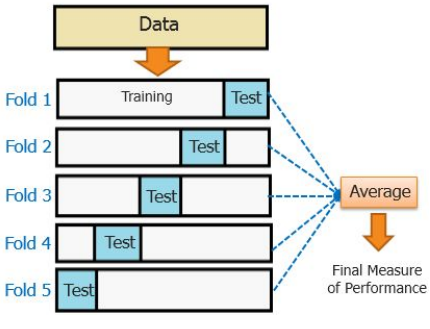
\includegraphics[width=.8\textwidth]{images/MobiDEV/6. activity recognition/cross validation.PNG}
    \end{center}
\end{minipage}

\subsection{Leave one subject out cross validation}
Simile alla cross-validation dove ad ogni fold, i dati di un utente vengono usati come test, i restanti utenti come training. Ad esempio se abbiamo 5 utenti, nel test abbiamo i dati di un utente, nel training i restanti 4.
Ogni fold usa come test un utente diverso infatti, abbiamo tante iterazioni quanti gli utenti.

\begin{minipage}{.55\textwidth}
    Il grafico ci fa vedere sull'asse x la complessità del modello, sull'asse y l'errore medio che il modello fa nella classificazione. La linea blu è il training error, un errore che fa il classificatore nel predirre l'attività sugli stessi dati del training. Più il modello è semplice e più l'errore è alto (high bias). Più andiamo a rendere il modello sofisticato più l'errore scende (hight variance)
    Cross-validation error rappresenta l'errore di predizione usando la cross-validation. 
    Lo scopo è di arrivare in un punto in cui minimizziamo l'errore sulla cross-validation error, cioè dove abbiamo dati che non abbiamo mai visto
\end{minipage} 
\hfill
\begin{minipage}{.45\textwidth}
    \begin{center}
        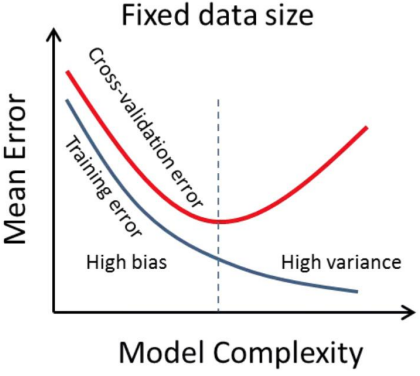
\includegraphics[width=.9\textwidth]{images/MobiDEV/6. activity recognition/leave one out.PNG}
    \end{center}
\end{minipage}

Possiamo avere due fenomeni:
\begin{itemize}
    \item \textbf{underfitting} che avviene con high bias: il modello è troppo semplice che non descrive sufficientemente i dati 
    \item \textbf{overfitting} che avviene con high variance: il modello calza a pennello con il training set, ma che fatica a generalizzare su dati mai visti
\end{itemize}
Entrambi i problemi vanno evitati.


\subsection{True/false positives/negatives}
Per ogni singola attività abbiamo i due set, training e test, e 
per valutare l'accuratezza di un classificatore è necessario calcolare (per ogni attività):
\begin{itemize}
    \item quante volte il classificatore ha calcolato l'attività A ed effettivamente l'utente ha fatto l'attività A (true positive)
    \item quante volte è stata predetta un'attività errata (false positive) 
    \item quante volte un'attività non è stata predetta (false negative)
\end{itemize}
Ad esempio prendiamo un sistema binario, che vuole capire quando sto saltando, dove accende la lampadina verde se salto. 
\begin{itemize}
    \item se salto e sto saltando è true positive
    \item se salto e non me lo dice è un falso negativo
    \item se sto fermo e dice che salto è un falso positivo
\end{itemize}

Partendo da TP, FP, FN, è possibile ricavare delle metriche per valutare la qualità di predizione del classificatore.
Le metriche più usate sono (hanno tutte un range tra 0 e 1, più la metrica va verso 1 più è buona, più tende allo 0 più sbaglia): \begin{itemize}
    \item precision: più è bassa e più sono presenti FP
    \begin{math}
        Precision = TP/(TP+FP)
    \end{math}
    Se il classificatore dice che corro sempre, la precision è bassa
    \item recall: più è bassa e sono presenti FN
    \begin{math}
        Recall = TP/(TP+FN)
    \end{math}
    Se il classificatore dice che corro sempre, la precision è alta
    \item F1: media armonica di precision e recall
    \begin{math}
        F1 = 2*(precision*recall)/(precision+recall)
    \end{math}
\end{itemize} 

\subsection{Matrice di confusione}
\begin{minipage}{.35\textwidth}
    È una matrice che ci fa capire quali attività possono essere confuse tra di loro.
    Le colonne rappresentano le attività predette dal sistema, le righe invece le volte in cui l'utente stava facendo effettivamente quell'attività. 
    In ogni cella abbiamo le volte in cui il sistema ha predetto l'attività ed effettivamente l'utente stava facendo quell'attività. 
    Nella diagonale principale abbiamo i TP e tutto ciò che sta fuori dalla diagonale, equivale ad un errore.
\end{minipage} 
\hfill
\begin{minipage}{.65\textwidth}
    \begin{center}
        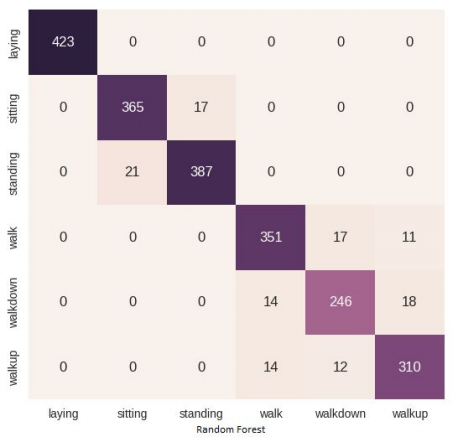
\includegraphics[width=.9\textwidth]{images/MobiDEV/6. activity recognition/matrice di confusione.PNG}
    \end{center}
\end{minipage}

\subsection{Tecniche di tuning}
Un modello di riconoscimento di attività ha tantissimi iper-parametri ed il tuning di questi valori non è banale.

Ci sono tecniche di tuning per cercare di trovare i valori che massimizzano il testing:
\begin{itemize}
    \item grid search: si provano delle combinazioni di iper-parametri, presi da elenchi di valori da testare, definiti dall'utente. È la tecnica utilizzata più spesso, ma computazionalmente pesante
    \item random search: sceglie in modo casuale delle combinazioni di iper-parametri, ma non dà garanzie sul miglior risultato
    \item bayesian optimization: tecnica di ottimizzazione sequenziale. Cerca di predire i valori di iper-parametri che massimizzi il miglioramento atteso. Costruisce un modello probabilistico per stimare i risultati attesi nello spazio degli iper-parametri
    Date le combinazioni di ip e dati i risultati sulle combinazioni di ip, vado a scegliere al prossimo giro una combinazione di ip che cerca di migliorare i risultati. Si continua iterativamente a selezionare iper-parametri fino alla convergenza
\end{itemize} 

\subsection{Recap. activity recognition con supervised learning}
\begin{enumerate}
    \item Raccolta dei dati per l'addestramento del sistema
    \item Pre-processing: definisco la tecnica e gli iper-parametri
    \item Etichettatura dei feature vector estratti dal pre-processing con le etichette raccolte
    \item Scelta dell'algoritmo di classificazione e dei relativi iper-parametri
    \item Validazione: calcolo la qualità del riconoscimento del classificatore
    \item Tuning: itero dal passo 2 (se necessario anche dal passo 1) per cercare di migliorare la qualità del riconoscimento
    \item Deploy: addestro il classificatore su tutto il dataset e lo sposto sul dispositivo mobile
\end{enumerate}

\section{Approcci semi-supervisionati per il riconoscimento di attività}
È poco pratico acquisire una grossa quantità di dati necessaria per ottenere un classificatore accurato.
Nei sistemi supervisionati il modello di attività viene creato una volta sola ed abbiamo due problemi:
\begin{itemize}
    \item ogni modello è fortemente dipendente da:
    \begin{itemize}
        \item persone, che hanno fornito i dati e come hanno svolto le attività
        \item attività considerate
    \end{itemize} 
    \item è necessario considerare un set limitato e pre-determinato di attività
    \item un soggetto può potenzialmente cambiare nel tempo il modo in cui svolge una specifica attività ed il modello iniziale può risultare non più accurato
\end{itemize} 

\subsection{Tecniche di apprendimento semi-supervisionato}
Sono tecniche di ML che permettono di inizializzare il classificatore con un dataset più ristretto, dopodiché si cerca di etichettare in maniera automatica i dati che non sono stati etichettati.
\\ Ci sono 3 tecniche principali:
\begin{itemize}
    \item self-training: abbiamo dataset ridotto x creare modello iniziale. Vogliamo usare il modello iniziale per propagare le etichette verso i dati non etichettati. 
    Abbiamo il dato non etichettato e il classificatore che con il modello iniziale applica il riconoscimento. L'output del classificatore viene associato come etichetta al dato non etichettato solo quando è sicuro che l'attività sia quella.
    I dati etichettati automaticamente vengono aggiunti al modello
    \item co-training: più classificatori vengono allenati su un piccolo dataset su diverse viste dei dati, ad esempio diversi feature vector, diverse porzioni del dataset. Il majority voting, tra i classificatori, determina la predizione su dati non etichettati. I dati etichettati dalla maggioranza vengono usati per aggiornare il modello
    \item active learning: uno dei metodi più efficaci ma non è una tecnica automatica. Richiede l'interazione con l'utente. Guarda quando il classificatore è poco sicuro su un'attività. In questo caso viene chiesta l'etichetta all'utente. L'etichetta viene poi usata per aggiornare il modello
\end{itemize}

Gli approcci hanno diversi limiti:
\begin{itemize}
    \item self-learning: gli errori nell'etichettatura automatica possono rinforzarsi col tempo
    \item co-training: più robusto del self-learning, ma può essere complicato creare più viste sensate dei dati
    \item active learning: sebbene sia una delle tecniche più potenti richiede un'interazione con l'utente per migliorare il modello
\end{itemize}

Le tecniche semi-supervised possono essere usate anche per creare un modello di attività che si personalizza sull'utente:
\begin{itemize}
    \item il modello iniziale viene creato da un insieme di 
    utenti diverso da quello finale
    \item l'utente finale scarica il modello e inizia ad usare il sistema
    \item con le tecniche semi-supervised, il modello viene aggiornato con dati etichettati dell'utente finale
\end{itemize}

Il training viene fatto una volta sola, perché una volta finito il modello non si aggiorna. Ogni volta che viene effettuato il training da capo, con i dati vecchi più le etichette nuove che abbiamo trovato, è time consuming e spesso impraticabile.
L'ideale è usale algoritmi di apprendimento incrementale, algoritmi il cui modello di attività viene aggiornato continuamente con nuovi esempi etichettati.

Esistono diversi tipi di algoritmi incrementali:
\begin{itemize}
    \item algoritmi nascono incrementali come k-NN, Linear Regression, Deep Learning
    \item ci sono estensioni di noti algoritmi in versione incrementale come SVM, Random Forest 
\end{itemize} 
